\documentclass[border={8pt 6pt 8pt 6pt}]{standalone}
% Gemeinsamer Preamble fuer die Standalone-Grafiken der Schlusspraesentation.
% Pakete gespiegelt aus src/thesis/hslu_thesis.tex (Z. 56-60), damit die
% extrahierten TikZ-/pgfplots-Grafiken identisch zur Arbeit rendern.
\usepackage[T1]{fontenc}
\usepackage[utf8]{inputenc}
\usepackage{tikz}
\usepackage{pgfplots}
\pgfplotsset{compat=1.18}
\usepgfplotslibrary{groupplots}
\usetikzlibrary{patterns}

\begin{document}
% Extrahiert 1:1 aus chapters/06_validation_und_evaluation.tex (fig:eval_results_overview).
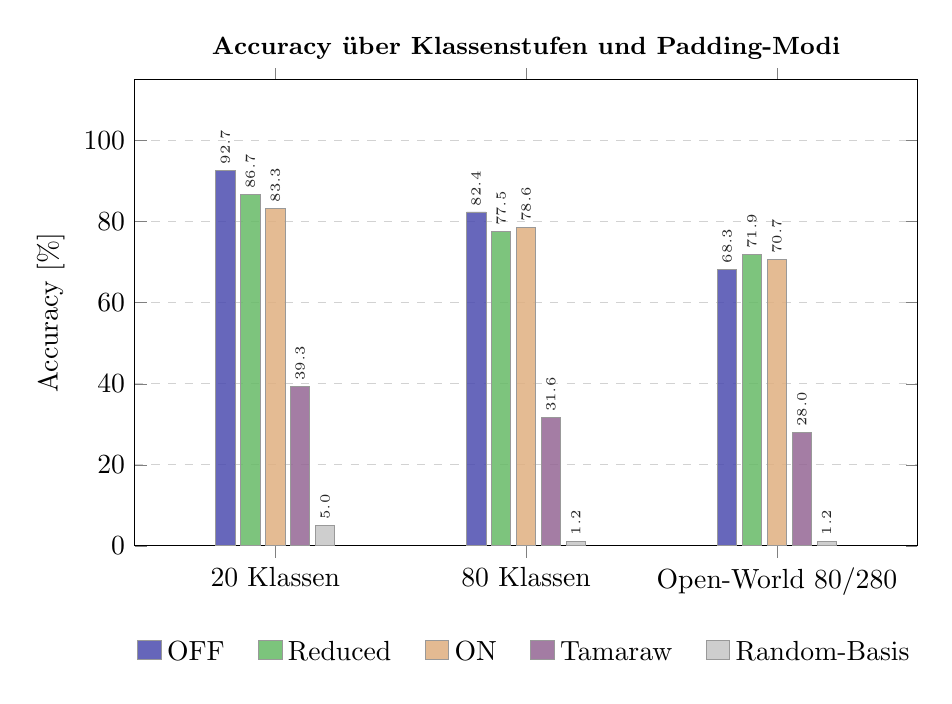
\begin{tikzpicture}
    \begin{axis}[
        ybar,
        title={Accuracy über Klassenstufen und Padding-Modi},
        title style={font=\small\bfseries, yshift=-2pt},
        width=0.95\textwidth,
        height=7.5cm,
        bar width=7pt,
        ymin=0, ymax=115,
        ylabel={Accuracy [\%]},
        symbolic x coords={20 Klassen, 80 Klassen, Open-World 80/280},
        xtick=data,
        enlarge x limits=0.28,
        ymajorgrids=true,
        grid style={dashed, gray!35},
        legend style={at={(0.5,-0.18)}, anchor=north, legend columns=5, draw=none, /tikz/every even column/.append style={column sep=10pt}},
        legend image code/.code={\draw[#1, draw=black!40, line width=0.3pt] (0cm,-0.08cm) rectangle (0.3cm,0.16cm);},
        nodes near coords,
        nodes near coords style={font=\tiny, rotate=90, anchor=west, inner sep=2pt, /pgf/number format/.cd, fixed, fixed zerofill, precision=1},
        every axis plot/.append style={fill opacity=0.85, draw=black!40, line width=0.3pt},
        tick style={black!50},
    ]
        \addplot[fill=blue!55!black!70]   coordinates {(20 Klassen,92.7) (80 Klassen,82.4) (Open-World 80/280,68.3)};
        \addplot[fill=green!55!black!60]  coordinates {(20 Klassen,86.7) (80 Klassen,77.5) (Open-World 80/280,71.9)};
        \addplot[fill=orange!75!black!50] coordinates {(20 Klassen,83.3) (80 Klassen,78.6) (Open-World 80/280,70.7)};
        \addplot[fill=violet!60!black!60] coordinates {(20 Klassen,39.3) (80 Klassen,31.6) (Open-World 80/280,28.0)};
        \addplot[fill=gray!45]            coordinates {(20 Klassen,5.0)  (80 Klassen,1.2)  (Open-World 80/280,1.2)};
        \legend{OFF, Reduced, ON, Tamaraw, Random-Basis}
    \end{axis}
\end{tikzpicture}
\end{document}
